\chapter{Literature Review: Software Testing}
\label{chap:softwareTesting}
The very famous quote of Paul, ``to err is human, but to really foul things up you need a computer", is quite relevant to the software programmers. Programmers being humans are prone to errors. Therefore, in spite of the best efforts, some errors may remain in the software after it is finalised.  Errors cannot be tolerated in software because a single error may cause a large upset in the system. The destruction of Mariner 1 rocket (1962) costing \$18.5 million was due to a small error in formula coded incorrectly by programmer. The Hartford Coliseum Collapse (1978) costing \$70 million, Wall Street crash (1987) costing \$500 billion, failing of long division by Pentium (1993) costing \$475 million, Ariane 5 Rocket disaster costing \$500 million and many others were caused by minor errors in the software \cite{toweysoftware}. To achieve high quality, a software has to satisfy rigorous stages of testing. The more complex the software, the higher the requirements for software testing and the larger the damage caused when a bug remains in the software.

\begin{figure}[h]
	\centering
	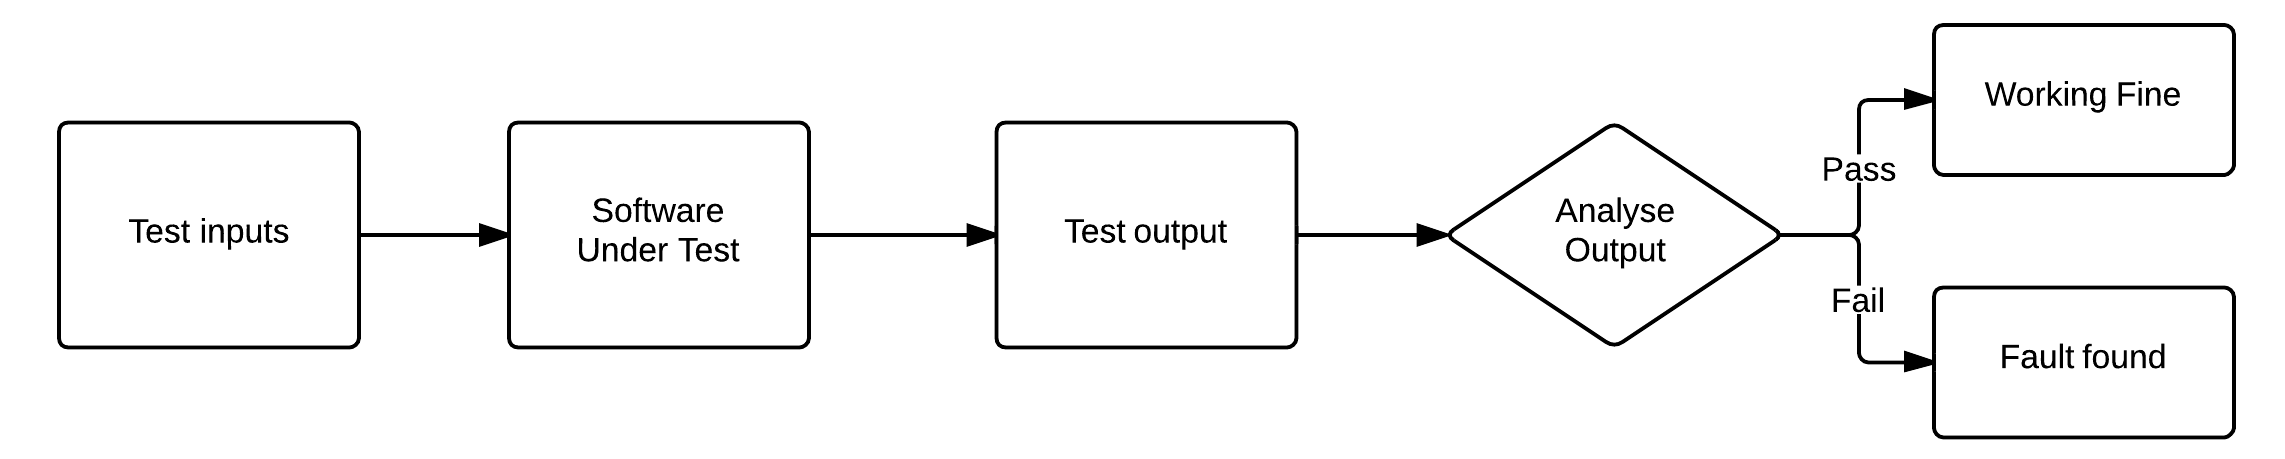
\includegraphics[width=15.5cm, height=4cm]{chapter2/softwareTesting.png}
	\caption{The process of software testing}
	\label{fig:softwareTesting}
\end{figure}

In the IEEE standard glossary of software engineering terminology~\cite{american1984}, testing is defined as ``the process of exercising or evaluating a system or system component by manual or automated means to verify that it satisfies the specified requirements and results". The process of software testing in its simplest form is shown in Figure~\ref{fig:softwareTesting}. A successful test is the one that fails a software or identify a fault in the sonftware~\cite{Myers1979}, where fault denotes the error made by programmers during software development~\cite{american1984}.

The testing process, being an integral part of Software Development Life Cycle (SDLC), is started from requirement phase and continues throughout the life of the software. In traditional testing when a tester finds a fault in the given SUT, the software is returned to the developers for rectification and is consequently given back to the tester for retesting. It is important to note that, ``program testing can be used to show the presence of bugs, but never to show the absence of bugs"~\cite{Dijkstra1972}. In other words, a SUT that passes all the tests without giving a single error is not guaranteed to contain no error. The testing process, however, increases reliability and confidence of users in the tested product. \\


\begin{table}[ht]
%\scriptsize
\caption{Parts of Software Testing} % title of Table
\smallskip
\centering % used for centering table
{\renewcommand{\arraystretch}{1.5} %<- modify value to suit your needs
\begin{tabular}{| l | l | l | l | } % centered columns (4 columns)
\hline

Levels 					&Purpose		 		& Perspective							& Execution 	\\
\hline
Unit						& Functional			& White Box							& Static 		\\
Integration				& Structural			& ~~~~~a. Data Flow Analysis				& Dynamic	\\
System					& Robustness			& ~~~~~b. Control Flow Analysis			&			\\
						& Stress				& ~~~~~c. Code-based fault injection testing 	&			\\
						& Compatibility			& Black Box							&			\\
						& Performance			& ~~~~~a. Use-case testing				&			\\
						&					& ~~~~~b. Partition testing				&			\\
						&					& ~~~~~c. Boundary Value testing			&			\\
						&					& ~~~~~d. Formal Specification testing		&			\\



\hline %inserts single line
\end{tabular}
}
\bigskip
\label{table:softwareTestingParts} % is used to refer this table in the text
\end{table}

\section{Definitions}
This section presents important definitions:

\subsection{Test Plan}
Test plan is a document which defines the goal, scope, method, resources and time schedule of testing \cite{futrell2001quality}. In addition, it includes the testable deliverables and the associated risk assessment. The test plan explains, {\it {who, when, why}} and {\it {how}} to perform a specific activity in the testing process. 

\subsection{Input Domain} 
The input domain comprises of all possible inputs for a software, including all the global variables, method arguments and the externally assigned variables, like keyboard inputs etc. For a given program P with input vector $ P =\{x1, x2, . . . , xn\}$, having $\{D1, D2, . . . , Dn\}$ as the domain of each input so that $x1 \in D1, x2 \in D2$ and so on. The domain D of a function is the cross product of the domains of each input: $D = D1 \times D2 \times . . . \times Dn$.

\subsection{Test Case}
%\begin{wrapfigure}{r}{0.35\textwidth}
%  \vspace{-20pt}
%  \begin{center}
%    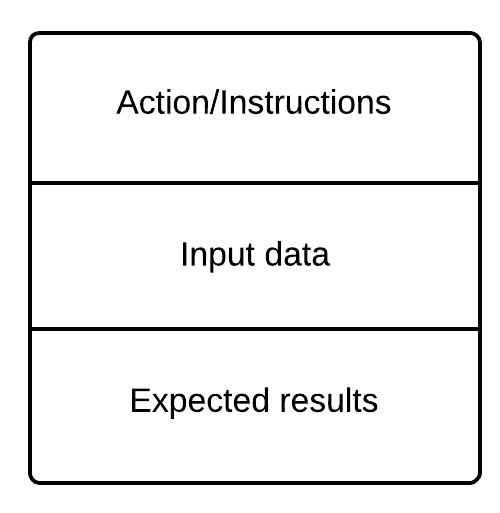
\includegraphics[width=0.30\textwidth]{chapter2/testCase.png}
%  \end{center}
%  \vspace{-20pt}
%  \caption{Test case}
%  \label{fig:testCase}
%  \vspace{-10pt}
%\end{wrapfigure}
A test case is an artifact which delineates the input, action and expected output corresponding to that input \cite{ahmed2010software}. After executing the test case, if the output obtained comply with the expected output, the test case is pass and the functionality is working correctly, otherwise the test case is fail, which represents identification of fault. Generally, a series of test cases, also known as test suite, are required to be executed for establishing the desired level of quality.

\section{Software Testing Levels}
Unit testing, integration testing and system testing are the three main levels of software testing reported in the literature~\cite{chilenski1994applicability}. Unit testing deals with evaluation of code piece-by-piece and each piece is considered as independent unit. Units are combined together to form components. Integration testing is performed to make sure that integration of units in a component is working properly. Finally, system testing ensures that the system formed by the combination of components proceeds properly to give the required output.

\section{Software Testing Purpose}
The primary purpose of software testing is identification of faults in the given SUT for necessary correction in order to achieve high quality. Maximum number of faults can be identified if software is tested exhaustively. In exhausting testing SUT is checked against all possible combinations of input data, and the results obtained are compared with the expected results for assessment. Exhaustive testing is not always possible in most scenarios because of limited resources and infinite number of input values that software can take. Therefore, the purpose of testing is generally directed to achieve confidence in the system involved from a specific point of view. For example, functionality testing is performed to check that functional aspect are working correctly. Structural testing analyses the code structure for generating test cases in order to evaluate paths of execution and identification of unreachable or dead code. In robustness testing the software behaviour is observed in the case when software receives input outside the expected input range. Stress and performance testing aims at testing the response of software under high load and checking its ability to process different nature of tasks~\cite{cohen2005robustness}. Finally, compatibility testing is performed to see the interaction of software with the underlying operating system.
 %As proper planning is the key to success for many projects this is often also true with software testing. A software test plan is a well defined document that defines the goal, scope, method, resources and time schedule of the testing.
%A software testing technique in which a software is tested with all possible combination of inputs. This technique can prove conclusively that the software meet its specification however exhaustive testing is seldom feasible because of the large input domain or too many paths in a software code. 

\section{Software Testing Perspective}
Software testing can be divided into white-box and black-box testing based on the perspective taken.

\subsection{White-box testing}
\begin{wrapfigure}{r}{0.36\textwidth}
  \vspace{-35pt}
  \begin{center}
    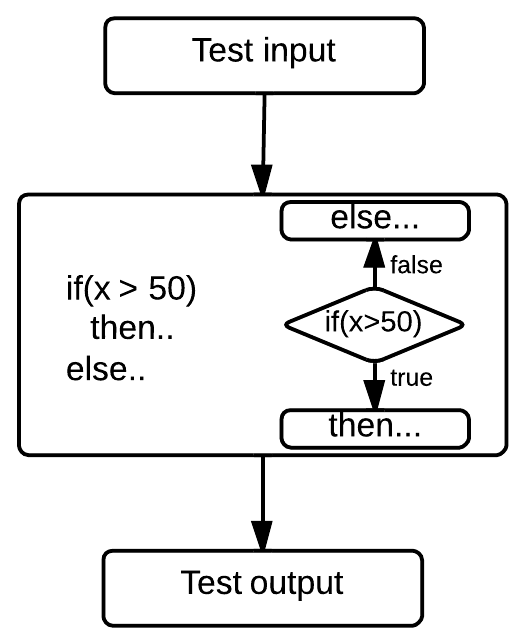
\includegraphics[width=0.30\textwidth]{chapter2/whiteBox.png}
  \end{center}
  \vspace{-20pt}
  \bigskip
  \caption{White-box testing}
  \label{fig:blackBox}
  \vspace{-18pt}
\end{wrapfigure}
In white-box or structural testing, the testers must know about the complete structure of the software so that they may make necessary modifications, if so required. Test cases are derived from the code structure and test passes only if the results are correct and the proper code is followed during test execution~\cite{ostrand2002white}. Some commonly used white-box testing techniques are as follows:

\subsubsection{Data Flow Analysis}
Data Flow Analysis (DFA) is a testing technique which focuses on the input values by observing the behaviour of respective variables during the execution of the SUT~\cite{clarke1989formal}. In this technique a Control Flow Graph (CFG), graphically representing all possible states of a program, drawn to determine the paths that are traversed by the program during its execution. Test cases are generated and executed to verify its conformance with CFG. 

Generally, program execution includes data input, its processing with the defined algorithm and output of results. The process can be looked into as data-flow from input to output where data may transform into several intermediary steps before reaching the final state. The process is prone to several errors e.g. references made to non existing variables, values assigned to undeclared variables or change of variables in undesired manner. Ordered use of data is crucial to ensure that the aforementioned errors do not occur~\cite{fosdick1976data}.

\subsubsection{Control Flow Analysis}
Control Flow Analysis (CFA) is a testing technique which takes into consideration the control structure of a given SUT. Control structure is the order in which the individual statements, instructions or function calls are executed. In this technique a CFG, similar to the one required in DFA, is drawn to determine the traversable paths by a program during the execution. Test cases are generated and executed to verify conformance with CFG on the basis of control. Taking the example of following a specific path between two or more available choices at a particular state: efforts are made to ensure that, at least once, the set of selected test cases execute all the possible control choices. The effectiveness of the testing technique depends on measurement of control. Two of the most common measurement criteria defined by Vilkomir et al. are Branch coverage and Condition coverage~\cite{vilkomir2003tolerance}. 

\subsubsection{Code-based fault injection testing}
It is a testing technique in which additional instructions are added to the code of the SUT at one or more locations to analyse the software behaviour in response to the anomaly \cite{voas1997software}. The process of code addition is called instrumentation which is performed before compilation and execution of software. Code is added for several reasons i.e. to find error handling behaviour of software by injecting faults, to examine the capability of test procedure with respect to the discovery of injected faults and to measure the code coverage achieved by the testing process.    

\subsection{Black-box testing}
\begin{wrapfigure}{r}{0.35\textwidth}
  \vspace{-35pt}
  \begin{center}
    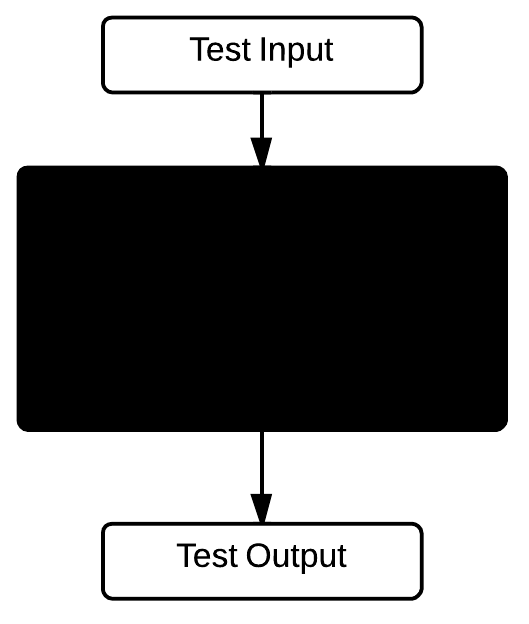
\includegraphics[width=0.30\textwidth]{chapter2/blackBox.png}
  \end{center}
  \vspace{-20pt}
  \bigskip
  \caption{Black-box testing}
  \label{fig:blackBox}
  \vspace{-18pt}
\end{wrapfigure}
In black-box or functional testing, the testers do not need to know about internal code structure of the SUT. Test cases are derived from the software specifications and test passes if the result is according to expected output~\cite{beizer1995black}. Some commonly used black-box testing techniques are stated below:

\subsubsection{Use-case based testing}
It is a verification and validation technique which utilizes use-cases of the system to generate test cases. Use-case defines functional requirement at a particular point in the system from actor's perspective. It consists of a sequence of actions to represent a particular behaviour of the system. A use-case format includes brief description and flow of events, preconditions, postconditions, extension points, context and activity diagrams. The use-case contains all the information required for test case, therefore, it can be easily transformed into a test case. Use-case testing is beneficial in terms of cheap generation of test cases, avoidance of test duplication, increased test coverage, easier regression testing and early identification of missing requirements.  

% steps taken from presentation of Raional User Conference 2003. Check it for viva.
\subsubsection{Partition Testing}
It is a testing technique in which the input domain of a given SUT is divided into sub-domains for testing each sub-domain individually. The division is based on software specifications, structure of the code and the process involved in software development \cite{hamlet1990}. The performance of partition testing is directly dependant on the quality of sub-domain \cite{weyuker1991analyzing}. However, division of input domain into equal partitions is often difficult. To overcome the problem, a new version of partition testing, called Proportional sampling strategy \cite{Chan1996} is devised. In this version, the sub-domains vary in size and the number of test cases selected from each partition is directly proportional to the size of the partition. Experiments performed by Ntafos~\cite{ntafos1998random} has provided experimental evidence for the better performance of Proportional partition testing.


\subsubsection{Boundary Value Analysis}
Boundary Value Analysis (BVA) is a testing technique based on the assumption that errors may often reside along the boundaries of the input variables. Thus border values are taken as the test data set in BVA. According to IEEE standards \cite{radatz1990ieee}, boundary value is a value that corresponds to minimum or maximum input, internal or external value specified for a system. 

The BVA technique and partition testing are also used simultaneously by choosing test values at the borders of each sub-domain as well as the whole input domain. Reid et al. \cite{reid1997empirical} have provided evidence in support of better performance of BVA compared to partition testing. However, they have indicated that better performance of BVA is based on accurate identification of partition and selection of boundary values.

 The following code illustrates the ability of BVA to find a bug.  On passing interesting value \verb+MAX_INT+ as argument to the $test$ method, the code in the method increment it by 1 making it a negative value and thus an error is generated when the system try to build an array of negative size.

\begin{lstlisting}
public void test (int arg) {
arg = arg + 1;
int [] intArray = new intArray[arg];
...
}
\end{lstlisting}



\subsubsection{Formal Specification Testing}
It is a testing technique based on mathematical model which provides the opportunity to handle the specifications mechanically. This feature facilitates the isolation, transformation, assembly and repackaging of the information available in the specifications for use as test cases~\cite{donat1997automating}.

The formal specification testing is more productive because of the creation of test cases independent from the code of the SUT~\cite{gaudel2010software}. The extra effort of generating test oracle is avoided because of using the available specification model for verifying the test results~\cite{bertolino2007software}.
  

%\section{Common Techniques of Software Testing}
%This section briefly define some of the most common techniques of software testing currently being used in the testing industry. These include techniques from both white-box and black-box testing techniques.

% Check wikipedia for them.


%\subsubsection{Grey-Box Testing}
%Grey-Box testing is the combination of both black-box/functionality and white-box/structural testing. The tester knows about both the functionality and the internal structure of the SUT. Some of the test cases are based on the functionality and some of the test cases are based on the structure. Emphasis of grey-box testing is both on code coverage as well as functionality~\cite{Savenkov2008}.

%\subsection{Software Testing Workflow}
%There are many software techniques like unit testing, integration testing, random testing, regression testing, system testing, acceptance testing, performance testing, load testing, stress testing, alpha testing, beta test etc. All testing techniques belong to black-box, white-box or grey-box approach. Each testing technique has its own strength and weaknesses but the technique in focus here is Random Testing.


%\begin{figure}[h]
%\begin{center}
%	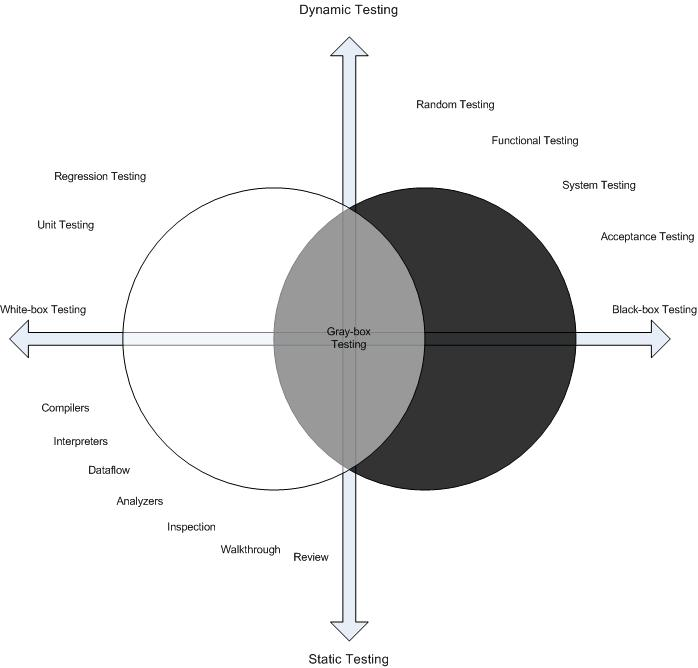
\includegraphics[width=16cm, height=12cm ]{Literature/Drawing34.jpg}
%	\caption{Software Testing Workflow}
%\end{center}  
%\end{figure}


%We have explained software testing graphically with the help of plotting venn diagram on two dimensional axis. The positive x axis represent black-box while negative x axis represent white-box testing. Grey-box testing in the middle is represented by the overlapping of black-box and white-box testing. Similarly on positive y axis we have dynamic testing and on negative y axis we have static testing.
%Now if a test is black box and dynamic then the test will fall in 0 to 90 degree on the diagram and if the test is black-box and static then it will fall in 270 to 360 degree. On the other hand if the test is white-box and dynamic then it will fall in 90 to 180 degree and if the test is white-box and static then it will fall in 180 to 270 degrees.

%\subsection{Automated Test Generation}
%\subsection{Generation Strategies}

\subsection{Test Oracle}
Test oracle is defined as, ``a source containing expected results for comparison with the actual result of the SUT" \cite{ahmed2010software}. According to Howden \cite{howden1986}, an oracle is a function which verifies if the output from program P is the same as the output from a ‘correct’ version of P. Test oracles set the acceptable behaviour for test executions~\cite{baresi2001test}. 

All software-testing techniques depend on the availability of test oracle~\cite{gaudel2010software}. Designing test oracle for ordinary software may be simple and straightforward. However, for relatively complex software designing of oracle is quite cumbersome and requires special ways to overcome the oracle problem. Some of the common issues associated with the orcale problem are as follows:
\begin{enumerate}
\item It is assumed that the test results are observable and comparable with the oracle.
\item Ideally, test oracle would satisfy desirable properties of program specifications~\cite{baresi2001test}.
\item A specific oracle to satisfy all conditions is seldom available as rightly pointed out by Weyuker, ``truly general test oracles are often unobtainable''~\cite{weyuker1982testing}. 
\end{enumerate}

Some of the most common artifacts used as oracles are stated below.
\begin{enumerate}
\item Specification and documentation to generate test oracle. 
\item Products similar to the SUT but different in algorithm to solve the similar problem.
\item Heuristic algorithms to provide exact results for a set of test cases. % Hoffman, Douglas; Heuristic Test Oracles, Software Testing & Quality Engineering Magazine, 1999
\item Statistical characteristics to generate test oracle. % \cite{mayer2004test}. 
\item Comparison of the result of one test to another for consistency. % Hoffman, Douglas; Analysis of a Taxonomy for Test Oracles, Quality Week, 1998
\item Models to generate test oracle for verification of SUT behaviour. % \cite{robinson1999finite}.
\item Manual analysis by human experts to verify the test results. %\cite{jalote1997integrated}. 
\end{enumerate}

\section{Software Test Execution}
Software test execution can be either static or dynamic. In static testing test cases are analysed statically for checking errors without test execution. Besides code, high quality softwares are supplied with documentation including requirements, design, user manual, technical and marketing information. Reviews, walkthroughs or inspections are most commonly used techniques for static testing. In dynamic testing the software code is executed and input is converted into output. Results are analysed against expected outputs to find any error in the software. Unit testing, integration testing, system testing, and acceptance testing are most commonly used as dynamic testing methods~\cite{fairley1978tutorial}.

%Dynamic testing can be manual or automated. In manual testing the programmer develops the test cases which are executed by the developed software to find any error in processing or output. Similarly in automated testing the software or components of the software is given as input to testing software that automatically generates test cases and executes the SUT against them to find any errors. Manual testing typically consumes more time and resources than automated testing.



\subsection{Manual Software Testing}
Manual testing is the technique of finding faults in software in which the tester writes the code by hand to create test cases and test oracle~\cite{Ciupa2008}. Manual testing may be effective in some cases but it is generally laborious, time consuming and error-prone~\cite{tretmans1999}. Additionally, it requires that the testers must have appropriate skills, experience and knowledge of the SUT for evaluation from different perspectives.
 
\subsection{Automated Software Testing}
Automated testing is the technique of finding faults in a software in which a testing tool is used to perform the testing process automatically~\cite{Leitner2007}. There are tools which can automate part of a testing process e.g. generation of test cases or execution of test cases or evaluation of results. Other tools are available which can automate the whole testing process. The increase in functionality, productivity and lower cost of production without compromising quality are the desirable features in favour of automating the process of software testing. Automated software testing can be very effective and highly beneficial for any organisation. Its initial cost may be higher, however, a quick return on investment outperforms it and brings the key benefits of cost reduction, higher productivity, availability, reliability and performance. Automated testing is particularly effective when the nature of job is repetitive and is performed on routine basis like unit testing and regression testing, where the tests are re-executed after each modification \cite{huang2003automated}. The use of automated software testing made it possible to test large volumes of code, which would have been impossible otherwise~\cite{ramamoorthy1975testing}.

\section{Test Data Generation}
Test data generation in software testing is the process of identifying test input data which satisfies the given test selection criterion. A test data generator tool is used to assist testers in the generation of test data while the test selection criterion define the properties of test cases to be generated based on the test plan and perspective taken \cite{korel1990}. Various artefacts of the SUT can be considered to generate test data like requirements, model, code etc. The choice of artefacts selected limits the kind of test selection criteria that can be applied in guiding the test case generation. 

A typical test data generator consists of three parts: Program analyser, Strategy Handler and Generator \cite{edvardsson1999survey}. Program analyser performs initial assessment of software prior to testing and may alter the code if so required. For example it performs code instrumentation or construction of CFG to measure the code coverage during testing. A strategy handler define the test case selection criteria. This may include the formalisation of test coverage criterion, the selection of paths, normalisation of constraints, etc. It may also get input from   program analyser or user before or during execution. The generator taking inputs from the program analyser and strategy handler generates test cases according to the set selection criteria.  Test data generators based on their approaches are classified into path-wise, goal-oriented, intelligent and random test. Each type is briefly described in the following section.

\subsection{Path-wise Test Data Generator}
It is a technique in which the test data is generated to target path, statement and branch coverage in a given SUT. The approach generally consists of three main parts: CFG construction, path selection and test data generation. 

In path-wise test data generation, the program path to the selected statement is identified and the input data are generated for evaluating the path which can be either generated automatically or provided by the user. The data generated in path testing expresses boolean behaviour i.e. true or false for a particular node in a path. 

A complete path contains multiple sub-domains, each sub-domain consists of test inputs required to traverse the path. The boundary of the sub-domains are obtained by the predicates in the path condition. The test data traversing a certain path in the software are selected from an input space split into a set of sub-sections. 

% the pathwise test data generation is taken from a book knowldge mining using intelligent systems. you can reference it too.


\subsection{Goal-oriented Test Data Generators}
It is a technique in which the test data is generated to target a specific program point rather than a program path \cite{chungautomated}. The tester can select any path among a set of existing paths as long as it reaches to the specified program point. This technique utilizes runtime information for computing accurate test data~\cite{ferguson1996chaining}. Among various methods used in goal-oriented test data generation the following two commonly adopted approaches are briefly described.

\subsubsection{Chaining Approach}
The chaining approach uses data dependent analysis to guide the test data generation. In the process all the related statement are selected automatically by the technique that are affected by the execution of the selected statement under test. The dependant statements are executed before the selected statement to generate the required necessary data for the execution of the statement under test~\cite{ferguson1996chaining}.

The chaining approach analyses the program according to the edges and nodes. For each test coverage criterion different initial event sequence and goal nodes are determined. For example, consider  the branch (p, q), where p is  the starting node of the branch and q is the last node in the branch. The initial event sequence E for the branch (p, q) is defined as $E =< (s,\phi), (p,\phi),(q,\phi) >$, provided that s is the starting node of the program and $\phi$ is the set of variables referred to as a constraint. The the Branch Classification process identifies critical, semi-critical and non-critical nodes for each branch. During the execution of the program, this classification leads the search to decide which branch to take to reach the goal node or to cover the specified branch.  


\subsubsection{Assertion-oriented Approach}
In this approach assertions are added to the program code with the goal to identify program input on which an assertion is violated, indicating a fault in the SUT. An assertion specifies a constraint that applies to some state of a computation which evaluates to either true or false. For example, consider a given assertion A, now find program input x on which assertion A is false, i.e. when the program is executed on input x and the execution reaches assertion A. It is evaluated as false indicating a fault in the SUT.

It is not always possible to generate test cases that violate assertions. However, experiments have shown that assertion-oriented test data generation may frequently detect errors in the program related to assertion violation. The major advantage of this approach is that each generated test data uncovers an error in the program with violation of an assertion. An assertion is violated because of three reasons: a faulty, a faulty assertion and a faulty precondition.

% check the korel1996assertion for the above whole text and assertion oriented approach + the model hard copy thesis.


\subsection{Intelligent Test Data Generators}
 Intelligent test data generation is a technique used to overcome the problems associated with traditional data generation techniques like generation of meaningless data, duplicated data and failing to generate complex test data. The approach increases users confidence in the generated test data and the testing process~\cite{ramamoorthy1975testing}. It performs sophisticated analysis, such as fuzzy logic, neural networks and genetic algorithms on the SUT to assist in finding the appropriate test data. It involves complex analysis to anticipate different situations that may arise at any point. The approach produces test data which satisfy the SUT requirements, however, it consumes more time and resources.

\subsubsection{Genetic Algorithm}
Genetic algorithm is a heuristic that mimics the evolution of natural species in searching for the optimal solution of a problem. The solution sought by the genetic algorithm is the test data that causes execution of a given statement, branch, path and condition in the SUT. The genetic algorithm is guided by control dependencies in the program to search for test data which satisfy test requirements. The genetic algorithm constructs new test data from previously generated test data. The algorithm evaluates the existing test data, and guide the direction of search by using the programs control-dependence graph \cite{pargas1999test}.

The benefit of the genetic approach is quick generation of test data with focus and direction. New test cases are generated by applying simple operations on existing test cases that are judged to have good potential of satisfying the test requirements. The success of this approach, however, depends heavily on the way in which the existing test data is measured \cite{pargas1999test}.

% Please paraphrase the above section genetic algorithm.

\subsection{Random Test Data Generators}

Random test data generator is the simplest technique for generation of test data. It has the advantage of being used to generate input data for any type of program. However, random test data generation is based solely on probability and cannot accomplish high coverage as its chances of finding semantically small faults are quite low [3find that reference].

If a fault is only revealed by a small percentage of the program input it is said to be a semantically small fault. For example of a semantically small fault consider the following code:
\begin{lstlisting}
void test(char x,char y) {
    if (x==y)
        System.out.println("Equal");
    else
        System.out.println("Not Equal");
}
\end{lstlisting}

It is easy to see that the probability of execution of the first statement is significantly lower than that of the second statement. As the structure gets complex so does the probability of its execution. Thus, such semantically small faults are hard to find by using random test data generation. 

\subsection{Search-based Test Data Generation}
It is a technique that uses meta-heuristic algorithms to guide generation of test data. In Search-based test data generation technique each input vector x can be associated with a measure $cost(x)$ that represents how far away the input vector x is from satisfying the set goal. Input test values closer to the set goal have low cost values and the other have high cost values. 

Consider a program with an initial branch statement: ${\it{ if (x >= 20) y = z; else y = 2 * z;}}$ and suppose we want the true branch to be executed. An input value of $x == 25$ clearly satisfies the predicate, and a value of $x == 15$ can be seen to come closer to satisfying the predicate than a value of $x ==5$. We might evaluate a cost function probe ( immediately before the indicated statement) of the form $cost(x) = max {0, 20 - x}$. Thus $x == 25$ has cost $0$, $x == 15$ has cost $5$ and $x = 5$ has cost $15$. We can see how finding data to satisfy the branch predicate is essentially a search over the input domain of x to find a value such that $cost(x) == 0$. 

Similarly, finding data to follow a particular path in the code can be considered as the one which satisfy each of the number of predicate at different points. This leads to a cost function which combines the costs at each of the relevant branching points. The approach requires the measurement of state at appropriate points in a programs execution. Moreover, the cost function plays the role of oracle for each targeted test requirement. Consequently, the cost function must change as per requirement. Frequent re-instrumentation of program is required to find test data that fully satisfy common coverage criteria. 

%At its heart search based software testing requires the use of search or optimisation algorithms. Most standard heuristic search techniques have been used, e.g. hill-climbing, simulated annealing, tabu search and genetic algorithms. 

% The details need not concern us here, and the reader is referred to McMinn [50] for details. Overall the search based 





%\subsection{Using A Model Checker}
%\subsection{Test Case Generation with Gatel by Using Lustre}
%\subsection{Using Models in Z}
%\subsectioin{Using UML Diagrams}
%\subsection{Using Misuse / Abuse Cases for Robustness Testing}
%\subsection{Randomly-generated test suites} % Dynamically discovering likely program invariants thesis page 77
%\subsection{Grammar-generated test suites Randomly}% Dynamically discovering likely program invariants thesis page 78
%\subsection{Test-case generation} %Combining over-and under-approximating program analysis for automatic software testing (section 4.2)
%\subsection{Mutation generation} % Automatic testing of software with structurally complex inputs. page 79 section 7.2.1
%\subsection{Test Data Generation} % page 70, 4.6.1, Coverage analysis for GUI Testing
% Check Generating Structurally complex tests from declarative constraints thesis 




% add diagram for generators similar to john paper in automated program flaw finding using simulated annealing.








%\section{Automated Random Testing}
%\subsection{Test Data Generation}
%\subsection{Test Execution}



%\subsection{Test Report}

\section{Summary}
The chapter gives an overview of software testing process, starting from defining what software testing is, why it is necessary, its common types and the purpose for which they are used. It then differentiate between manual and automated software testing and finally various ways of software test data generation, being the most critical and crucial part of any testing system are studied.


% ------------------------------------------------------------------------


%%% Local Variables:
%%% mode: latex
%%% TeX-master: "../thesis"
%%% End:
